\documentclass[11pt,oneside,a4paper]{article}
\usepackage{graphicx}
\usepackage{booktabs}
\usepackage{caption}
\usepackage{subcaption}
\usepackage{amsmath}
\usepackage{amsfonts}
\usepackage{amssymb}
\usepackage{lscape}
\usepackage{psfrag}
\usepackage[usenames]{color}
\usepackage{bbm}
\usepackage[update]{epstopdf}
\usepackage[bookmarks,pdfstartview=FitH,a4paper,pdfborder={0 0 0}]{hyperref}
\usepackage{verbatim}
\usepackage{listings}
\usepackage{textcomp}
\usepackage{course}
\usepackage{fancyhdr}
\usepackage{multirow}
\usepackage{algorithm}
\usepackage{algcompatible}
\usepackage[noend]{algpseudocode}
\pagestyle{fancy}
\usepackage{tikz}
\usepackage{xcolor}

\renewcommand{\sectionmark}[1]{\markboth{#1}{#1}}
\renewcommand{\subsectionmark}[1]{\markright{#1}}

\fancyhf{}
\fancyhead[RO]{\nouppercase{\footnotesize\sc\leftmark\ \hrulefill\ \thepage}}
\fancyhead[RE]{\nouppercase{\footnotesize\sc\thepage\ \hrulefill\ }}
\renewcommand{\headrulewidth}{0pt}

\makeatletter
\def\cleardoublepage{\clearpage\if@twoside \ifodd\c@page\else%
\hbox{}%
\thispagestyle{empty}%
\clearpage%
\if@twocolumn\hbox{}\clearpage\fi\fi\fi}
\makeatother


\renewcommand{\topfraction}{0.9}  % max fraction of floats at top
\renewcommand{\bottomfraction}{0.8} % max fraction of floats at bottom
% Parameters for TEXT pages (not float pages):
\setcounter{topnumber}{2}
\setcounter{bottomnumber}{2}
\setcounter{totalnumber}{4}            % 2 may work better
\setcounter{dbltopnumber}{2}           % for 2-column pages
\renewcommand{\dbltopfraction}{0.9}    % fit big float above 2-col. text
\renewcommand{\textfraction}{0.07}     % allow minimal text w. figs
% Parameters for FLOAT pages (not text pages):
\renewcommand{\floatpagefraction}{0.7}  % require fuller float pages
% N.B.: floatpagefraction MUST be less than topfraction !!
\renewcommand{\dblfloatpagefraction}{0.7} % require fuller float pages

\sloppy

\widowpenalty=10000
\clubpenalty=10000

\edef\today{%\number\day\
\ifcase\month\or
January\or February\or March\or April\or May\or June\or July\or
August\or September\or October\or November\or December\fi\ \number\year}
\title{\vspace*{40.0mm}
  \bf\sf Parallel Hashing
         \vspace*{20.0mm} \\
  \vspace*{40.0mm}
  %\vspace{-20mm}\framebox{DRAFT VERSION}\vspace{20mm} \\
  \Large\bf\sf Program for Undergraduate Research \vspace*{20.0mm}}
\author{\sf Kamer Kaya, Fatih Tasyaran,Kerem Yildirir,Hakan Ogan Alpar,Ali Osman Berk}
\date{\sf \today}

\begin{document}

\begin{figure}
  \parbox[t]{40mm}{
    \begin{flushleft}
      
\includegraphics[height=25mm]{pure.png}
    \end{flushleft}}
    \hspace{7cm}
  \parbox[t]{40mm}{
    \begin{flushright}
      
\includegraphics[height=25mm]{sabanj.png}
    \end{flushright}}
\end{figure}

\maketitle
\thispagestyle{empty}
\raggedbottom

\cleardoublepage
\pagenumbering{roman}
\setcounter{tocdepth}{2}
\tableofcontents


\section{Introduction}
\par Hash functions are 
\section{Intel SIMD Instructions}
SIMD is an instruction set available mostly on all current processors. In this project we used AVX(Advanced Vector Extension) and AVX2 instructions which are available for Intel processors since Sandy Bridge architecture. With AVX instructions, it is possible to process 128 bits of data in registers on parallel, with AVX2 this increased to 256 bits. The SIMD instructions we used on this project and their descriptions could be found in the following paragraph.

\subsection{Load-Extract Instructions}
\textcolor{blue}{\_\_m256i} \mm256\_load\_si256 (\textcolor{blue}{\_\_m256i const *} \textcolor{green}{mem\_addr})
\par Load 256-bits of integer data from memory into dst.mem\_addr must be aligned on a 32-byte boundary.
\par
\textcolor{blue}{\_\_m256i} \mm256\_loadu\_si256 (\textcolor{blue}{\_\_m256i const *} \textcolor{green}{mem\_addr})
\par Load 256-bits of integer data from memory into dst.mem\_addr does not need to be aligned on any particular boundary.
\par
\textcolor{blue}{ \_\_int32} \_mm256\_extract\_epi32 ( \textcolor{blue}{ \_\_m256i} \textcolor{green}{a}, \textcolor{blue}{const int} \textcolor{green}{b})
\par Add 4 packed to 256-bit side by side 64-bit integers in a and b, and store the results in dst.
\par
\textcolor{blue}{ \_\_m256i} \_mm256\_set1\_epi32 ( \textcolor{blue}{ int} \textcolor{green}{a})
\par Broadcast 32-bit integer a to all elements of dst.
\par 
\subsection{Bitwise Instructions}
\textcolor{blue}{ \_\_m256i} \_mm256\_slli\_epi64 ( \textcolor{blue}{ \_\_m256i} \textcolor{green}{a}, \textcolor{blue}{int} \textcolor{green}{imm8})
\par Shift packed 64-bit integers in a left by imm8 while shifting in zeros, and store the result in dst.
\par
\textcolor{blue}{ \_\_m256i} \_mm256\_slri\_epi64 ( \textcolor{blue}{ \_\_m256i} \textcolor{green}{a}, \textcolor{blue}{int} \textcolor{green}{imm8})
\par Shift packed 64-bit integers in a right by imm8 while shifting in zeros, and store the result in dst.
\par
\textcolor{blue}{ \_\_m256i} \_mm256\_shuffle\_epi32 ( \textcolor{blue}{ \_\_m256i} \textcolor{green}{a}, \textcolor{blue}{int} \textcolor{green}{imm8})
\par Shuffle 32-bit integers in a within 128-bit lanes using the control in imm8, and store the results in dst.
\subsection{Arithmetic Instructions}
\textcolor{blue}{ \_\_m256i} \_mm256\_add\_epi32 ( \textcolor{blue}{ \_\_m256i} \textcolor{green}{a}, \textcolor{blue}{ \_\_m256i} \textcolor{green}{b})
\par Add 8 packed to 256-bit side by side 32-bit integers in a and b, and store the results in dst.
\par
\textcolor{blue}{ \_\_m256i} \_mm256\_add\_epi64 ( \textcolor{blue}{ \_\_m256i} \textcolor{green}{a}, \textcolor{blue}{ \_\_m256i} \textcolor{green}{b})
\par Add 4 packed to 256-bit side by side 64-bit integers in a and b, and store the results in dst.
\par
\textcolor{blue}{ \_\_m256i} \_mm256\_sub\_epi64 ( \textcolor{blue}{ \_\_m256i} \textcolor{green}{a}, \textcolor{blue}{ \_\_m256i} \textcolor{green}{b})
\par Subtract packed 64-bit integers in b from 64-bit integers in a, and store the result in dst.
\par
\textcolor{blue}{ \_\_m256i} \_mm256\_mullo\_epi32 ( \textcolor{blue}{ \_\_m256i} \textcolor{green}{a}, \textcolor{blue}{ \_\_m256i} \textcolor{green}{b})
\par Multiply the packed 32-bit integers in a and b, producing intermediate 64-bit integers, and store the low 32 bits of the intermediate integers in dst.
\par
\subsection{Logical Instructions}
\textcolor{blue}{ \_\_m256i} \_mm256\_and\_si32 ( \textcolor{blue}{ \_\_m256i} \textcolor{green}{a}, \textcolor{blue}{ \_\_m256i} \textcolor{green}{b})
\par Compute the bitwise AND of 256 bits integer represented data in a and b and store the result in dst.
\par
\textcolor{blue}{ \_\_m256i} \_mm256\_xor\_si256 ( \textcolor{blue}{ \_\_m256i} \textcolor{green}{a}, \textcolor{blue}{ \_\_m256i} \textcolor{green}{b})
\par Compute the bitwise XOR of 256 bits integer represented data in a and b and store the result in dst.
\par

\section{Hashing Functions}
We have developed our work under 2 models; Model 1, one data multiple hash, where we generate multiple hash values from a single data sample, and Model 2, one data one hash, where we generate only one hash value using the same random seed for a single data sample. As our hash functions, we used Multiply-Shift Hash, MurMurHash3  and Tabular Hash. 
\subsection{Model 1}
\begin{figure}[H]
\centering
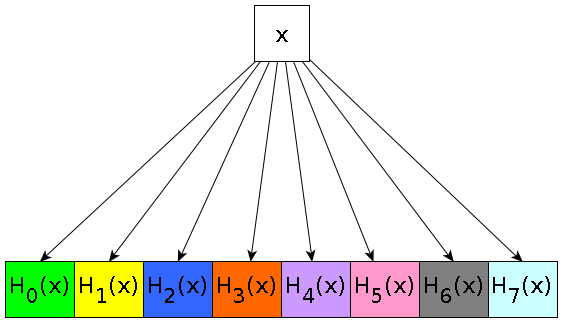
\includegraphics[width=0.5\textwidth]{one_data_multi_hash.png} 
\end{figure}
\subsection{Model 2}
\begin{figure}[H]
\centering
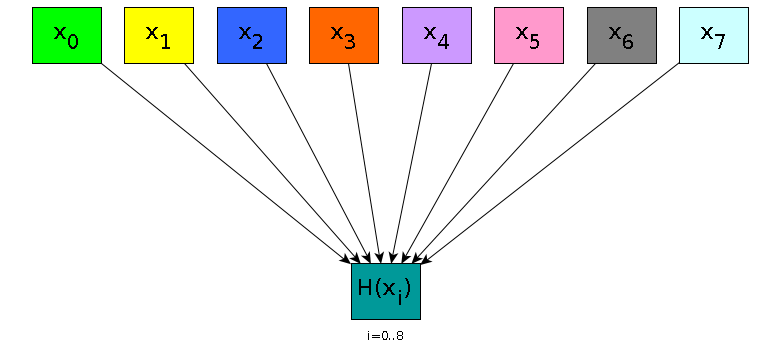
\includegraphics[width=0.7\textwidth]{multi_data_single_hash.png} 
\end{figure}
\subsection{Multiply-Shift Hash}
\begin{algorithm}[H]
\begin{algorithmic}[1]
\Function {Multiply-Hash}{x}

\State{2 randomly sampled 64 bit integers $m_a$,$m_b$ ; }


\Return {$(m_a*(uint\_64)*x + m_b ) >> 32$}
\EndFunction
\end{algorithmic}


\end{algorithm}



\subsection{MurMurHash3}
\begin{algorithm}[H]
\begin{algorithmic}[1]
\Function{Murmur3}{key, len, seed}
   % //Note: In this version, all integer arithmetic is performed 
    %//with unsigned 32 bit integers. In the case of overflow, 
   % //the result is constrained by the application 
%    //of modulo 232 arithmetic.

    \State c1 = 0xcc9e2d51
    \State c2 = 0x1b873593
    \State r1 = 15
    \State r2 = 13
   \State  m = 5
    \State n = 0xe6546b64

    \State hash  =  seed

    \For {each fourByteChunk of key}
         \State  k ← fourByteChunk

          \State k = k * c1
          \State k = (k ROL r1)
          \State k = k * c2

          \State hash = hash XOR k
          \State hash = (hash ROL r2)
          \State hash = hash * m + n
	\EndFor        
	
	 \Comment{ Endian swapping is only necessary on big-endian machines.}

   \For {each remaining byte in key}

  \State      remainingBytes = SwapEndianOrderOf(remainingBytesInKey)

         \State  remainingBytes = remainingBytes * c1
          \State remainingBytes = (remainingBytes ROL r1)
          \State remainingBytes = remainingBytes * c2

         \State  hash = hash XOR remainingBytes
\EndFor
      \State hash = hash XOR len

     \State  hash = hash XOR (hash SHR 16)
      \State hash = hash * 0x85ebca6b
      \State hash = hash XOR (hash SRH 13)
      \State hash = hash * 0xc2b2ae35
      \State hash = hash XOR (hash SHR 16)
    \EndFunction
\end{algorithmic}
\end{algorithm}

\subsection{Tabular Hash}
\section{Experiment and Results}
\section{Future Work}
\subsection{HyperLogLog}
\subsection{Bloom Filter}
\subsection{Count-Min Sketch}
\section{Conclusions}
\cleardoublepage
\pagenumbering{arabic}

\cleardoublepage


\bibliographystyle{ieeetr}
\bibliography{mybib.bib}
\end{document}
